\begin{table}[t]
\centering
\small
\setlength{\tabcolsep}{3pt}
\resizebox{\columnwidth}{!}{%
\begin{tabular}{@{}lcccc@{}}
\toprule
\textbf{Method} & \textbf{Seed 42} & \textbf{Seed 123} & \textbf{Seed 456} & \textbf{Mean} \\
\midrule
Uniform                & 17.694 & 17.686 & 17.702 & 17.697 $\pm$ .008 \\
Adaptive $\bstar$ (ours) & \textbf{17.680} & \textbf{17.666} & \textbf{17.677} & \textbf{17.674} $\pm$ .006 \\
ESS-only               & 17.730 & 17.720 & 17.760 & 17.737 $\pm$ .021 \\
Random $\mathcal{U}(0,2)$ & 17.830 & 17.800 & 17.777 & 17.802 $\pm$ .027 \\
Permuted $q$-scores  & 17.919 & --     & --     & 17.919 \\
\bottomrule
\end{tabular}}
\caption{Main comparison: held-out PPL ($\downarrow$) at $\rho{=}0.4$, 1 content epoch.
Adaptive and Uniform: 5-seed means (seeds 42, 123, 456, 789, 234); ESS-only and Random: 3-seed means (seeds 42, 123, 456); Permuted: single seed (42).
Adaptive uses $\tau{=}0.7$, $\nmin{=}2$.
Permuted randomly shuffles $q$-scores across samples, destroying provenance signal while preserving weight non-uniformity ($\Delta{=}{+}0.225$).}
\label{tab:main}
\end{table}

\subsection{Main Results}
\label{sec:main-results}

Table~\ref{tab:main} reports held-out perplexity at $\rho = 0.4$ across five seeds.
Continued pretraining reduces PPL from 22.970 to the 17.3--17.8 range; method comparisons operate within a narrow residual.

Adaptive $\bstar$ achieves 5-seed mean PPL 17.674, compared to 17.697 for uniform ($\Delta{=}{-}0.023$, directionally consistent across all seeds) and 17.620 for grid $b{=}0.3$ (3-seed mean, post-hoc oracle; gap $+$0.054; Table~\ref{tab:aux}).
A paired $t$-test yields $t(4){=}{-}8.21$, $p{=}0.0012$; after Bonferroni--Holm correction for nine family-wise comparisons, $p_{\mathrm{BH}}{=}0.011$, reaching conventional significance at $\alpha{=}0.05$.
The engineering benefit is eliminating $b$ grid search (nine full training runs~\citep{drayson2025detection}, ${\sim}$16 GPU-hours at 0.6B scale, scaling linearly with model size), though grid search yields a larger improvement.
The grid-best $b{=}0.3$ is a post-hoc oracle from nine candidates with ${\sim}6{\times}$ higher cross-seed standard deviation than adaptive ($\sigma{=}0.035$ vs.\ $0.006$); the noisy PPL plateau at $b \in [0.1, 0.5]$ (Figure~\ref{fig:grid_b_trend}) makes validation-based selection unreliable.
At the nearest fixed point ($b{=}1.0$), PPL equals uniform (17.692 vs.\ 17.694): per-batch adaptation is essential.

The ablation hierarchy at $\rho{=}0.4$ (Adaptive ${<}$ Uniform ${<}$ ESS-only ${<}$ Random ${<}$ Permuted, Table~\ref{tab:main}) reveals two requirements for effective reweighting: detector signal and minimum intervention.
Random weights $\mathcal{U}(0,2)$ (17.802) confirm that non-uniform weighting alone does not help; permuted $q$-scores (17.919, $\Delta{=}{+}0.225$) further isolate provenance signal as load-bearing, since shuffling destroys the detector's sample-level information while preserving identical weight non-uniformity.
ESS-only (mean $17.737 {\pm} 0.021$) uses the same $q$-scores but maximizes $b$ up to the stability ceiling, concentrating weights on a few high-confidence samples; it degrades PPL by 0.043 relative to uniform.
Only the dual-constrained adaptive method, which limits $b$ to the minimum needed, improves in-distribution PPL over uniform (mean $\Delta{=}{-}0.023$, directionally consistent across all seeds).
Figure~\ref{fig:grid_b_trend} contextualizes both results: adaptive $\bstar$ operates near the curve minimum while ESS-only $\bstar$ (mean ${\approx}$3.5) falls in the degradation zone.

\begin{figure}[t]
\centering
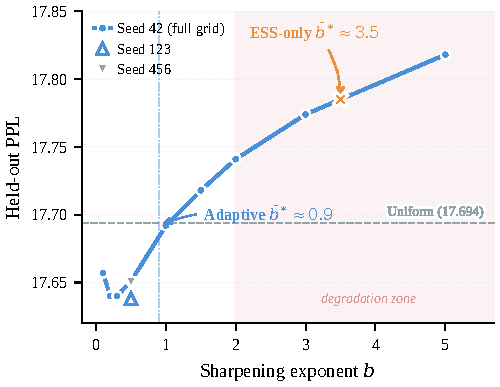
\includegraphics[width=\columnwidth]{grid_b_trend_clean}
\caption{Held-out PPL as a function of fixed sharpening exponent $b$ (grid search, $\rho{=}0.4$).
Seed\,42 provides the full nine-point sweep (circles); cross-seed markers at $b{=}0.5$ (triangles) confirm the plateau region.
The shaded region marks $b \geq 2$ where PPL degrades past the uniform baseline; ESS-only $\bstar$ (overall mean ${\approx}$3.5) falls in this degradation zone, while adaptive $\bstar$ (mean ${\approx}$0.9) operates near the curve minimum.}
\label{fig:grid_b_trend}
\end{figure}

\paragraph{Hard filtering and multi-epoch exposure.}
Detect \& Remove at its best threshold ($q{>}0.3$) achieves 3-seed mean PPL $17.250 \pm 0.001$ at full training length, outperforming all reweighting methods by a wide margin ($\Delta{=}{-}0.424$ vs.\ adaptive $\bstar$).
All three D\&R thresholds beat both uniform and adaptive $\bstar$ ($q{>}0.5$: $17.280 \pm 0.010$; $q{>}0.7$: $17.320 \pm 0.001$; 3 seeds each), with cross-seed variance near zero (holdout $\pm$0.00, Table~\ref{tab:epoch_match}).
Aggressive filtering retains only 31.5\% of tokens at $q{>}0.3$, so the model sees surviving data ${\sim}$3.2 \emph{content epochs} versus one for reweighting; an epoch-matched control (D\&R at $q{>}0.5$, ${\sim}$1.0 content epochs) yields PPL $17.657 \pm 0.005$ vs.\ $17.674 \pm 0.007$ for adaptive $\bstar$ ($\Delta{=}0.017$), attributing ${>}$95\% of D\&R's full-length advantage to multi-epoch exposure on filtered data (Table~\ref{tab:epoch_match}).
This decomposition identifies the \emph{mechanism}: filtering concentrates compute on high-confidence real data, and multi-epoch exposure amplifies the benefit, rather than undermining D\&R's practical effectiveness.
The raw threshold--PPL curve is U-shaped ($q{>}0.3$: 17.25, $q{>}0.9$: 17.42), but epoch-matched comparisons eliminate the U-shape, revealing monotonically decreasing PPL that saturates at $q{\geq}0.5$ (Figure~\ref{fig:dr_dual_curve}; Appendix~\ref{app:hybrid}).
For practitioners, D\&R is the strongest strategy when the corpus is small relative to training compute, as aggressive filtering naturally creates multi-epoch regimes that amplify quality gains; controlled comparisons should report the effective content-epoch count alongside PPL.

\begin{figure}[t]
\centering
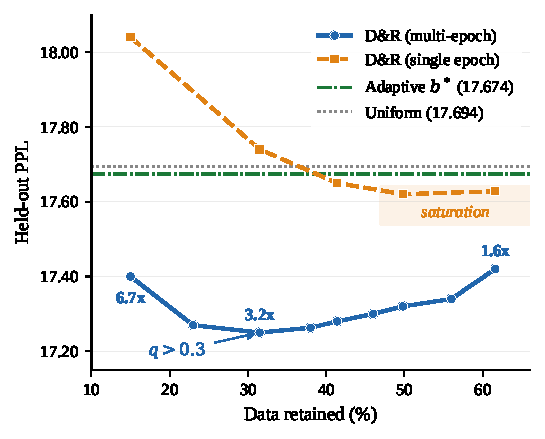
\includegraphics[width=\columnwidth]{dr_dual_curve}
\caption{D\&R threshold--PPL relationship ($\rho{=}0.4$, 3 seeds).
Blue: raw (multi-epoch) PPL with effective epoch counts annotated.
Orange: epoch-matched PPL (single content epoch), saturating at the adaptive $\bstar$ level (green dashed).}
\label{fig:dr_dual_curve}
\end{figure}

\begin{figure}[t]
\centering
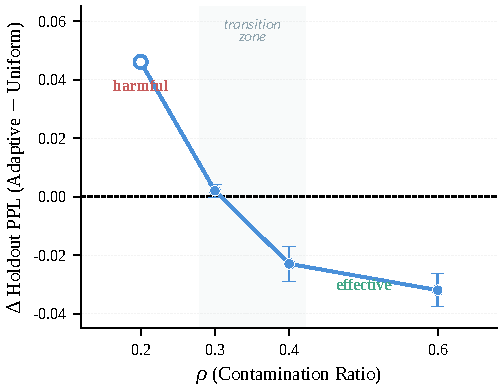
\includegraphics[width=\columnwidth]{delta_vs_rho}
\caption{Effect of contamination ratio on adaptive reweighting effectiveness.
$\Delta$ = adaptive $-$ uniform holdout PPL (lower is better).
Error bars show $\pm$1 SD across seeds.
The method transitions from harmful to beneficial between $\rho{=}0.3$ and $0.4$ (shaded).}
\label{fig:delta_vs_rho}
\end{figure}

\subsection{Robustness and Boundary Conditions}
\label{sec:robustness}

Across three seeds at $\rho = 0.6$, adaptive $\bstar$ ($17.731 \pm 0.004$) directionally outperforms uniform on in-distribution PPL ($17.763 \pm 0.008$, $\Delta{=}{-}0.032$, 3 seeds, paired $t{=}{-}9.95$, $p_{\mathrm{BH}}{=}0.064$), with a larger effect size than at $\rho{=}0.4$ ($\Delta{=}{-}0.023$).
The ablation hierarchy is preserved (Grid 17.634\footnote{Single seed; full per-seed results in Appendix~\ref{app:rho06}.} ${<}$ Adaptive 17.731 ${<}$ Uniform 17.763 ${\approx}$ ESS-only 17.765 ${<}$ Random 17.861), but the ESS-only/uniform gap collapses to effectively zero ($17.763$ vs.\ $17.765$) as ESS binding rises to ${\sim}$49\%.
Random remains substantially worse than uniform (gap 0.098, $\sigma{=}0.027$): detector signal is load-bearing even when the stability constraint dominates; the adaptive method's continued advantage is driven by the $\aeff$ quality constraint, which operates independently of the ESS ceiling.
Three-seed paired comparison confirms $\tau{=}0.7$ outperforms $\tau{=}0.8$ on both holdout and out-of-distribution (OOD) metrics (\S\ref{sec:sensitivity}).

\begin{table}[t]
\centering
\small
\setlength{\tabcolsep}{3pt}
\resizebox{\columnwidth}{!}{%
\begin{tabular}{@{}lccc@{}}
\toprule
\textbf{Method} & \textbf{Epochs} & \textbf{PPL (raw)} $\downarrow$ & \textbf{PPL (ep.-matched)} $\downarrow$ \\
\midrule
D\&R ($q{>}0.3$) & ${\sim}$3.2 & \textbf{17.250} $\pm$ .001 & 17.74 \\
D\&R ($q{>}0.5$) & ${\sim}$2.4 & 17.280 $\pm$ .010 & 17.657 $\pm$ .005 \\
D\&R ($q{>}0.7$) & ${\sim}$2.0 & 17.32 & 17.62 \\
\midrule
Adaptive $\bstar$ & ${\sim}$1.0 & \multicolumn{2}{c}{17.674 $\pm$ .007} \\
Uniform           & ${\sim}$1.0 & \multicolumn{2}{c}{17.697 $\pm$ .008} \\
\bottomrule
\end{tabular}}
\caption{D\&R threshold comparison ($\rho{=}0.4$).
Raw PPL traces a U-shape across thresholds; epoch-matched PPL (single content epoch) decreases monotonically and saturates near the adaptive $\bstar$ level.
D\&R's 0.424 PPL advantage (at $q{>}0.3$) shrinks to $\Delta{=}0.017$ when content epochs are equalized.
All raw PPL values are 3-seed means; epoch-matched values at $q{>}0.3$ and $q{>}0.7$ are single-seed.
Full 9-threshold sweep in Table~\ref{tab:dr_threshold}.}
\label{tab:epoch_match}
\end{table}

\paragraph{Scale.}
At 1.7B parameters (Qwen3-1.7B, $\rho{=}0.4$, $\tau{=}0.8$, 3 seeds), the method scales without degradation but the benefit diminishes.
Adaptive $\bstar$ achieves holdout PPL $13.26$ vs.\ uniform $13.27$ ($\Delta{=}{-}0.013$); OOD results are mixed in direction across domains (OWT $\Delta{=}{-}0.008$, Wiki $\Delta{=}{+}0.013$) and downstream accuracy is unchanged ($\Delta{\approx}{+}0.002$).
The diminished effect is consistent with larger models being more robust to self-generated contamination: Qwen3-1.7B's own outputs are likely closer to its training distribution, reducing the distributional shift that reweighting corrects.
A preliminary Llama-3.2-3B cross-model result (Appendix~\ref{app:cross_model}) shows mixed downstream effects (MMLU $+$1.6 percentage points, HellaSwag $-$0.6 percentage points), leaving cross-architecture generalization as an open question.
\paragraph{Out-of-distribution evaluation.}
To test whether the in-distribution improvement reflects distribution matching, we evaluate all three from-scratch seeds on OpenWebText and Wikipedia.
At $\rho{=}0.4$, adaptive reweighting improves mean PPL on all three evaluation domains: FineWeb $\Delta{=}{-}0.023$ (5 seeds), OpenWebText $\Delta{=}{-}0.026$, Wikipedia $\Delta{=}{-}0.027$ (3 seeds each); downstream accuracy is near-identical (0.5414 vs.\ 0.5415).
OOD improvements exceed the in-distribution gain, indicating genuine quality improvement rather than distribution matching toward the training mixture ($\tau{=}0.8$'s OOD effect is smaller; $\tau{=}0.7$'s advantage reflects active OOD improvement, \S\ref{sec:sensitivity}).

\paragraph{Calibration, not just discrimination.}
Replacing TF-IDF+LR with generative perplexity detectors reverses the advantage across three seeds (GPT-2: AUC\,=\,0.91, ECE\,=\,0.131, $\Delta{=}{+}0.098$; N-gram: AUC\,=\,0.73, ECE\,=\,0.069, $\Delta{=}{+}0.129$; Figure~\ref{fig:overview}b; Appendix~\ref{app:detector}).
The TF-IDF vs.\ GPT-2 contrast (comparable AUC, $2.7{\times}$ ECE gap) isolates calibration as an empirically observed requirement in our self-contamination setting; N-gram's better ECE (0.069) does not compensate for insufficient AUC (0.73), indicating that both discrimination and calibration are jointly necessary (Figure~\ref{fig:overview}b).

\begin{table}[t]
\centering
\small
\setlength{\tabcolsep}{3pt}
\resizebox{\columnwidth}{!}{%
\begin{tabular}{@{}lcccl@{}}
\toprule
\textbf{Method} & \textbf{Seeds} & \textbf{Oracle?} & \textbf{Epochs} & \textbf{Mean PPL} $\downarrow$ \\
\midrule
Grid ($b{=}0.3$) & 3 & post-hoc & 1 & \textbf{17.620} $\pm$ .033 \\
Golden Ratio     & 1 & known $\rho$ & 1 & 17.654 \\
D\&R ($q{>}0.3$) & 3 & post-hoc & ${\sim}$3.2 & \textbf{17.250} $\pm$ .001 \\
\bottomrule
\end{tabular}}
\caption{Auxiliary baselines at $\rho{=}0.4$. Grid-best selected post-hoc from nine candidates (Appendix~\ref{app:grid}). Golden Ratio requires known $\rho$~\citep{he2025golden}. D\&R uses ${\sim}$3.2 content epochs (Table~\ref{tab:epoch_match}).}
\label{tab:aux}
\end{table}

\subsection{Hyperparameter Sensitivity}
\label{sec:sensitivity}

\paragraph{Quality threshold $\tau$.}
$\tau{=}0.7$ outperforms $\tau{=}0.8$ on holdout at both contamination levels ($\rho{=}0.4$: 17.674 vs.\ 17.683; $\rho{=}0.6$: paired $t{=}{-}4.70$, $p{<}0.05$; \S\ref{sec:robustness}) and achieves larger OOD gains ($\rho{=}0.4$: $\Delta{=}{-}0.026$/$-$0.027 vs.\ $-$0.003/$-$0.002; Table~\ref{tab:tau}, Appendix~\ref{app:tau_rho}).
$\tau \in [0.5, 0.8]$ all improve holdout over uniform, while $\tau {>} 0.8$ degrades (Appendix~\ref{app:tau_sweep}).
We also tested per-batch adaptive $\tau$ clamping, which did not improve over fixed thresholds (Appendix~\ref{app:batch_adaptive}).

\paragraph{ESS floor $\nmin$.}
The default $\nmin{=}2$ ($\nmin/B{=}0.5$) is optimal; extremes degrade ($\nmin{=}1$: PPL $17.742{\pm}0.009$, 3 seeds, worse than uniform; $\nmin{=}B$: recovers uniform).
Neither constraint alone improves over uniform ($\nmin{=}1$: $+$0.048; ESS-only: $+$0.043); both must act jointly for the method to outperform uniform training.
The coupling $\nmin{=}\lfloor B/2 \rfloor$ is also empirically motivated: at $B{=}8$, keeping $\nmin{=}2$ (ratio $0.25$) degrades PPL by $+$0.036 vs.\ uniform, whereas $\nmin{=}4$ (ratio $0.5$) yields $\Delta{=}{-}0.052{\pm}0.007$.
Under this coupling, the adaptive advantage monotonically increases across $B \in \{4, 8, 16\}$: $\Delta{=}{-}0.023{\pm}0.006$ (5 seeds), $-$0.052${\pm}$0.007 (3 seeds, $p{=}0.006$), and $-$0.068${\pm}$0.005 (3 seeds), corresponding to $1.0{\times}$, $2.3{\times}$, and $3.0{\times}$ amplification ($p{<}0.01$ at $B \geq 8$).
The gap to grid-best narrows from 0.040 ($B{=}4$) to 0.009 ($B{=}16$, seed\,42; Figure~\ref{fig:batch_amp}).

\begin{figure}[t]
\centering
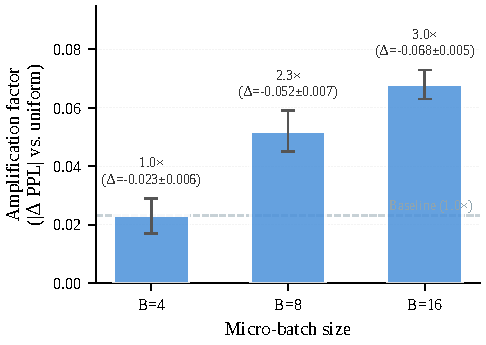
\includegraphics[width=\columnwidth]{batch_size_amplification}
\caption{Batch-size amplification of adaptive reweighting ($\nmin{=}\lfloor B/2 \rfloor$).
The adaptive advantage over uniform increases monotonically with micro-batch size, from $1.0{\times}$ ($B{=}4$) to $3.0{\times}$ ($B{=}16$); $\Delta$ values and $\pm$1\,SD shown above each bar.}
\label{fig:batch_amp}
\end{figure}

\paragraph{Constraint regime.}
\label{sec:regime}
Over 24{,}412 micro-batches (seed\,42), 5.8\% are clean ($\aeff(0) \geq \tau$, $\bstar{=}0$), ${\sim}$50\% are $\aeff$-binding (quality constraint dominates), and ${\sim}$44\% are ESS-binding (stability constraint dominates); the distribution is stable across seeds (coefficient of variation ${<}2\%$; Figure~\ref{fig:regime_decomp}).
The $\aeff$-binding majority indicates that detector quality signal, not training stability, is the primary bottleneck, reinforcing the calibration requirement (\S\ref{sec:robustness}).

\begin{figure}[t]
\centering
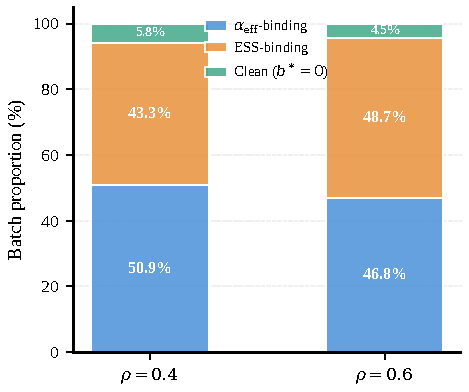
\includegraphics[width=\columnwidth]{constraint_regime_decomposition}
\caption{Constraint regime decomposition at two contamination levels (seed\,42).
At $\rho{=}0.4$, ${\sim}$50\% of batches are $\aeff$-binding and ${\sim}$44\% ESS-binding, with ${\sim}$6\% clean; at $\rho{=}0.6$, the constraints are nearly balanced (${\sim}$49\% ESS-binding, ${\sim}$47\% $\aeff$-binding).}
\label{fig:regime_decomp}
\end{figure}
